\newpage
\section{Cursor}
    In diesem Kapitel wird der Cursor mit allen Funktionen und Bestandteilen erläutert.
    Darunter fallen unter anderem eine Variable (cursorColumn, deklariert in Viergewinnt.asm, Größe 1 Byte)
    zur Beschreibung der horizontalen-Position auf dem Board. Sie repräsentiert die Spalte, die durch den Cursor ausgewählt wird.
    Weiterhin eine Konstante (cursorRow, in Viergewinnt.asm deklariert, hat den Wert 6) für die vertikale-Position des Cursors direkt unterhalb des Spielfelds.

    \subsection{Aufbau}
        Der Cursor wird auf dem LCD durch einen 6 Byte Breiten, ausgefüllten Pfeil unter dem Spielfeld (Zeile 6) dargestellt (Abbildung \ref{fig:cursor}).

        \begin{figure}[H]
            \centering
            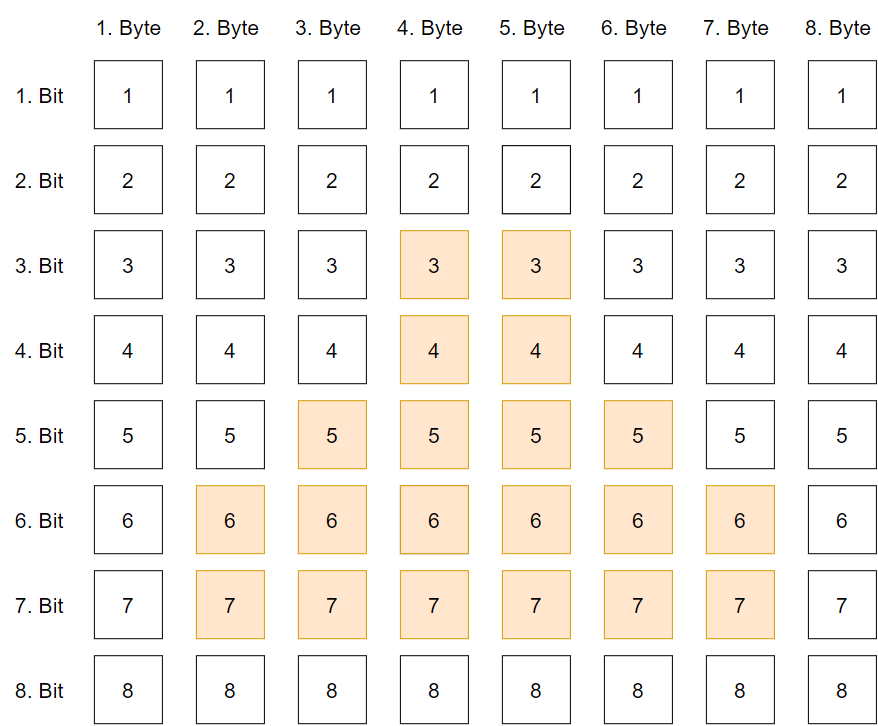
\includegraphics[scale=0.35]{img/cursor.png}    
            \caption{Cursor auf dem LCD}
            \label{fig:cursor}
        \end{figure}
    
    \subsection{Steuerung}
        Der Cursor startet nach betätigen des Resets (Taste 4 des Boards) oder bei Programmstart in der Mitte des Spielfeldes (Spalte 4).
        Er kann durch die Tasten 1 (nach links) und 3 (nach rechts) horizontal unter dem Spielfeld bewegt werden.+
        Bei weiterer Bewegung und einer Cursorposition am Spielfeldrand erscheint der Cursor am gegenüberliegenden Spielfeldrand um schnelleres manövrieren zu ermöglichen (Abbildung \ref{fig:board}).
        \\
        Bei Versersetzen des Cursors wird zuerst auf dem LCD der alte Cursor gelöscht,
        dann die Variable cursorColumn für links um 1 reduziert oder für rechts um 1 erhöht.
        Danach wird der Cursor erneut auf dem LCD an der geänderten cursorColumn angezeigt.

        \begin{figure}[H]
            \centering
            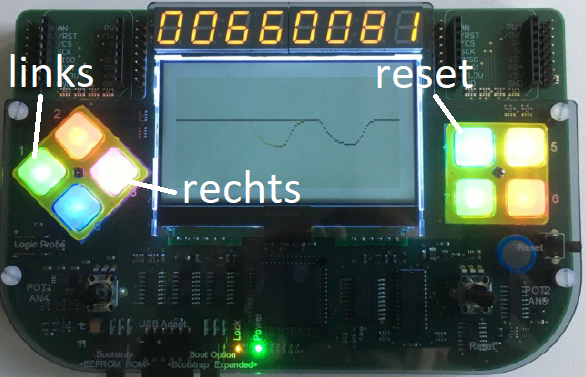
\includegraphics[scale=0.5]{img/board.png}    
            \caption{Board}
            \label{fig:board}
        \end{figure}